\documentclass[12pt,a4paper]{article}

\usepackage[margin=1in]{geometry}
\usepackage{amsmath}
\usepackage{amssymb}
\usepackage{booktabs}
\usepackage{array}
\usepackage{hyperref}
\usepackage{float}
\usepackage{xcolor}
\usepackage{listings}
\usepackage{graphicx}
\usepackage{tikz}
\usepackage{pgfplots}

\pgfplotsset{compat=1.18}
\usetikzlibrary{positioning}

\hypersetup{
    colorlinks=true,
    linkcolor=blue,
    urlcolor=blue,
    citecolor=blue
}

\lstset{
    basicstyle=\ttfamily\small,
    breaklines=true,
    frame=single,
    backgroundcolor=\color{gray!8}
}

\title{\textbf{Multi-Level Parking Assignment Optimization}}
\author{Optimization Project}
\date{}

\begin{document}

\maketitle

\begin{abstract}
This report presents a dynamic multi-level parking assignment optimization model. A real smart-parking dataset is used to estimate demand characteristics, while a synthetic multi-level parking structure is generated to satisfy the project requirement of modeling floors, capacities, space attributes, and walking distances. Four solution approaches are implemented and compared: greedy assignment, genetic algorithm, simulated annealing, and integer linear programming. The implemented constraints include vehicle assignment, time-aware space capacity, size compatibility, EV charging requirements, floor capacity, dynamic arrival/departure behavior, and unassigned-vehicle penalties. Experimental results show that the ILP gives the best offline benchmark solution, while simulated annealing and genetic algorithms improve over the greedy baseline.
\end{abstract}

\section{Introduction}

This project studies the assignment of vehicles to parking spaces in a multi-level parking facility. Vehicles arrive over time and must be assigned to available and compatible spaces. The goal is to reduce user inconvenience while satisfying operational constraints such as space capacity, size compatibility, electric vehicle charging requirements, and dynamic arrival/departure behavior.

The inconvenience considered in this project is mainly based on walking distance to the exit, with penalties for vehicles that cannot be assigned. The problem is solved and compared using four methods: a greedy online algorithm, a genetic algorithm, simulated annealing, and an integer linear programming model.

\section{Problem Description}

The parking facility consists of several floors. Each floor contains a fixed number of parking spaces. Each space has attributes such as size, floor, position, and whether it has an electric vehicle charger.

Each vehicle is characterized by:

\begin{itemize}
    \item arrival time,
    \item parking duration,
    \item departure time,
    \item vehicle type,
    \item required size category,
    \item whether it requires electric charging.
\end{itemize}

The objective is to assign vehicles to spaces while minimizing the total assignment cost and respecting all feasibility constraints.

\section{Project Requirements Coverage}

Table~\ref{tab:requirements} summarizes how the implementation matches the requested project requirements.

\begin{table}[H]
\centering
\caption{Coverage of Project Requirements}
\label{tab:requirements}
\resizebox{\textwidth}{!}{
\begin{tabular}{lll}
\toprule
Requirement & Status & Implementation Description \\
\midrule
Multi-level parking structure & Included & 3 floors with 20 spaces per floor \\
Parking spaces with attributes & Included & Floor, position, size, EV charger availability \\
Vehicle set with attributes & Included & Arrival time, duration, type, size need, EV charging need \\
Walking distance matrix & Included & Synthetic internal distance matrix and exit-distance vector \\
Vehicle assigned exactly once & Included & Assignment or unassigned dummy variable \\
One vehicle per space at a time & Included & Time-overlap constraints and dynamic repair procedures \\
Size compatibility & Included & Compact/SUV/van hierarchy \\
EV charging requirement & Included & EVs requiring charging must use charger spaces \\
Floor capacity & Included & Enforced through physical space capacity \\
Dynamic arrivals/departures & Included & Arrival and duration used by all solvers \\
Ramp/elevator access capacity & Partial & Stored as a parameter, not enforced as hard constraint \\
Congestion & Partial & Simplified; reported through peak floor occupancy \\
\bottomrule
\end{tabular}
}
\end{table}

\section{Dataset and Synthetic Instance Generation}

The project uses the recommended smart parking dataset from Kaggle:

\begin{center}
\url{https://www.kaggle.com/datasets/datasetengineer/smart-parking-management-dataset}
\end{center}

The dataset contains information such as vehicle type, electric vehicle status, parking duration, occupancy rate, entry time, spot size, and parking status.

Since the dataset does not include a multi-level parking structure, a synthetic parking infrastructure was generated. The dataset is used to estimate demand characteristics, while the parking structure is generated artificially.

The generated benchmark instance contains:

\begin{itemize}
    \item multiple parking floors,
    \item a fixed number of spaces per floor,
    \item size categories for parking spaces,
    \item electric vehicle charging spaces,
    \item synthetic walking distances to the exit,
    \item generated vehicles with arrival times and durations.
\end{itemize}

All random generation is controlled using a fixed seed to ensure reproducibility.

\begin{figure}[H]
\centering
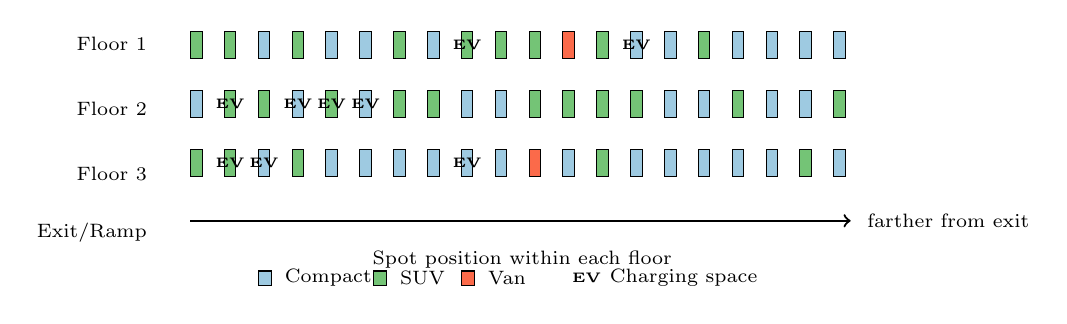
\begin{tikzpicture}[x=0.43cm,y=0.75cm, font=\scriptsize]
    \definecolor{compactColor}{RGB}{158,202,225}
    \definecolor{suvColor}{RGB}{116,196,118}
    \definecolor{vanColor}{RGB}{251,106,74}

    \newcommand{\spot}[4]{
        \pgfmathsetmacro{\cx}{#1+0.17}
        \pgfmathsetmacro{\cy}{#2+0.225}
        \draw[fill=#3, draw=black, line width=0.35pt] (#1,#2) rectangle ++(0.34,0.45);
        \node at (\cx,\cy) {#4};
    }

    \node[anchor=east] at (0,3.25) {Floor 1};
    \node[anchor=east] at (0,2.15) {Floor 2};
    \node[anchor=east] at (0,1.05) {Floor 3};
    \node[anchor=east] at (0,0.05) {Exit/Ramp};

    \foreach \x in {3,5,6,8,14,15,17,18,19,20} {\spot{\x}{3}{compactColor}{}}
    \foreach \x in {1,2,4,7,9,10,11,13,16} {\spot{\x}{3}{suvColor}{}}
    \foreach \x in {12} {\spot{\x}{3}{vanColor}{}}
    \foreach \x in {9,14} {\node[font=\tiny\bfseries] at (\x+0.17,3.225) {EV};}

    \foreach \x in {1,4,6,9,10,15,16,18,19} {\spot{\x}{2}{compactColor}{}}
    \foreach \x in {2,3,5,7,8,11,12,13,14,17,20} {\spot{\x}{2}{suvColor}{}}
    \foreach \x in {2,4,5,6} {\node[font=\tiny\bfseries] at (\x+0.17,2.225) {EV};}

    \foreach \x in {3,5,6,7,8,9,10,12,14,15,16,17,18,20} {\spot{\x}{1}{compactColor}{}}
    \foreach \x in {1,2,4,13,19} {\spot{\x}{1}{suvColor}{}}
    \foreach \x in {11} {\spot{\x}{1}{vanColor}{}}
    \foreach \x in {2,3,9} {\node[font=\tiny\bfseries] at (\x+0.17,1.225) {EV};}

    \draw[->, thick] (1,0.25) -- (20.5,0.25);
    \node[anchor=west] at (20.7,0.25) {farther from exit};
    \node[anchor=north] at (10.8,-0.1) {Spot position within each floor};

    \draw[fill=compactColor, draw=black] (3,-0.85) rectangle ++(0.4,0.25);
    \node[anchor=west] at (3.5,-0.72) {Compact};
    \draw[fill=suvColor, draw=black] (6.4,-0.85) rectangle ++(0.4,0.25);
    \node[anchor=west] at (6.9,-0.72) {SUV};
    \draw[fill=vanColor, draw=black] (9.0,-0.85) rectangle ++(0.4,0.25);
    \node[anchor=west] at (9.5,-0.72) {Van};
    \node[font=\tiny\bfseries] at (12.7,-0.72) {EV};
    \node[anchor=west] at (13.1,-0.72) {Charging space};
\end{tikzpicture}
\caption{Synthetic multi-level parking structure generated for the benchmark instance. Each row is a floor and each rectangle is a parking space. The colors represent space size categories and the ``EV'' label indicates a charging-equipped space.}
\label{fig:layout}
\end{figure}

\section{Implemented Constraints}

This section describes the constraints that are explicitly taken into account in the implementation.

\subsection{Vehicle Assignment Constraint}

Each vehicle must be assigned to exactly one parking space, or marked as unassigned if no feasible space is available.

Let $x_{vs}$ be a binary variable equal to 1 if vehicle $v$ is assigned to space $s$, and 0 otherwise. Let $y_v$ be a binary variable equal to 1 if vehicle $v$ is unassigned.

\begin{equation}
\sum_{s \in S} x_{vs} + y_v = 1 \qquad \forall v \in V
\end{equation}

This guarantees that a vehicle cannot be assigned to multiple spaces.

\subsection{Parking Space Capacity Over Time}

Each parking space can accommodate at most one vehicle at a time. However, since the problem is dynamic, the same parking space can be reused by another vehicle after the first vehicle departs.

For two vehicles $v_1$ and $v_2$, their parking intervals overlap if:

\begin{equation}
\max(a_{v_1}, a_{v_2}) < \min(d_{v_1}, d_{v_2})
\end{equation}

where $a_v$ is the arrival time and $d_v$ is the departure time.

If two vehicles overlap in time, they cannot be assigned to the same space:

\begin{equation}
x_{v_1s} + x_{v_2s} \leq 1
\qquad
\forall s \in S,\ \forall (v_1,v_2) \text{ overlapping}
\end{equation}

This is one of the most important constraints because it makes the model time-aware.

\subsection{Size Compatibility Constraint}

Each vehicle can only be assigned to a space that is large enough. The size hierarchy used is:

\begin{equation}
\text{compact} < \text{suv} < \text{van}
\end{equation}

Therefore:

\begin{itemize}
    \item compact vehicles can use compact, SUV, or van spaces,
    \item SUV vehicles can use SUV or van spaces,
    \item van vehicles can only use van spaces.
\end{itemize}

If a vehicle does not fit in a space, that assignment is forbidden:

\begin{equation}
x_{vs} = 0
\qquad
\text{if vehicle } v \text{ is too large for space } s
\end{equation}

\subsection{Electric Vehicle Charging Constraint}

Electric vehicles that require charging must be assigned to parking spaces equipped with chargers.

If vehicle $v$ requires charging and space $s$ does not have a charger, the assignment is forbidden:

\begin{equation}
x_{vs} = 0
\qquad
\text{if } v \text{ requires charging and } s \text{ has no charger}
\end{equation}

If no charger-equipped space is available at the required time, the vehicle may be marked as unassigned and receives a penalty in the objective function.

\subsection{Floor Capacity Constraint}

Each floor has a fixed number of physical parking spaces. Since each physical space can contain at most one vehicle at a time, floor capacity is automatically respected.

For example, if a floor contains 20 spaces, then at most 20 vehicles can be assigned simultaneously to that floor.

\subsection{Dynamic Arrival and Departure Constraint}

Vehicles arrive and depart dynamically. A space occupied by a vehicle is unavailable until that vehicle's departure time. After departure, the space becomes available again.

This dynamic behavior is considered in:

\begin{itemize}
    \item the greedy algorithm,
    \item the genetic algorithm repair procedure,
    \item the simulated annealing repair procedure,
    \item the ILP overlap constraints.
\end{itemize}

\subsection{Unassigned Vehicle Penalty}

If a vehicle cannot be assigned to any feasible space, it is marked as unassigned and receives a penalty in the objective function. This avoids producing infeasible solutions while still making unassignment undesirable.

\begin{equation}
\text{Penalty Cost} = P \sum_{v \in V} y_v
\end{equation}

\section{Constraints Not Fully Modeled}

The project statement also mentions access constraints, such as ramp or elevator capacity. In the current implementation, ramp capacity exists as an instance parameter, but it is not enforced as a hard optimization constraint.

Congestion is also modeled in a simplified way. The greedy solver includes a basic congestion component, and floor occupancy is reported during evaluation. However, a detailed traffic-flow congestion model is left as future work.

Therefore, the implemented constraints are:

\begin{itemize}
    \item vehicle assignment,
    \item parking space capacity over time,
    \item size compatibility,
    \item EV charging requirement,
    \item floor capacity,
    \item dynamic arrival and departure,
    \item unassigned vehicle penalty.
\end{itemize}

The partially included or future-work constraints are:

\begin{itemize}
    \item ramp/elevator access capacity,
    \item detailed congestion modeling.
\end{itemize}

\section{Objective Function}

The objective is to minimize total user inconvenience. In the implemented model, this is represented mainly by walking distance and unassigned vehicle penalties.

\begin{equation}
\min \sum_{v \in V} \sum_{s \in S} c_{vs} x_{vs}
+ P \sum_{v \in V} y_v
\end{equation}

where:

\begin{itemize}
    \item $c_{vs}$ is the cost of assigning vehicle $v$ to space $s$,
    \item $P$ is the penalty for leaving a vehicle unassigned,
    \item $x_{vs}$ is the vehicle-space assignment variable,
    \item $y_v$ is the unassigned vehicle variable.
\end{itemize}

The main component of $c_{vs}$ is the walking distance from the parking space to the exit.

\section{Algorithms Implemented}

\subsection{Greedy Algorithm}

The greedy algorithm is an online method. It processes vehicles in arrival order. For each arriving vehicle, it checks all currently available compatible spaces and assigns the best one.

This method is fast and realistic for real-time systems, but it does not have future knowledge.

\subsection{Genetic Algorithm}

The genetic algorithm is a population-based metaheuristic. Each chromosome represents preferred parking assignments for all vehicles. Since random assignments can be infeasible, a repair procedure is applied to ensure that time, size, and EV constraints are respected.

The genetic algorithm uses:

\begin{itemize}
    \item an initial population,
    \item tournament selection,
    \item crossover,
    \item mutation,
    \item elitism,
    \item repair and evaluation.
\end{itemize}

\subsection{Simulated Annealing}

Simulated annealing is a local search method. It starts from an initial solution and repeatedly modifies it. Worse moves can be accepted with a probability that decreases over time. This helps the algorithm escape local minima.

The implemented simulated annealing method starts from the greedy solution, applies random assignment changes, repairs the solution, and keeps the best solution found.

\subsection{Integer Linear Programming}

The ILP model is an exact offline optimization method. It assumes that all arrivals and departures are known in advance. It provides a benchmark solution for comparing the heuristic methods.

The ILP explicitly includes binary variables, assignment constraints, compatibility constraints, EV charger constraints, and time-overlap constraints.

\section{Experimental Results}

The experiment was run using the following instance:

\begin{itemize}
    \item 3 floors,
    \item 20 spaces per floor,
    \item 60 total spaces,
    \item 60 vehicles,
    \item seed = 42,
    \item 7 EV vehicles,
    \item 9 EV-capable spaces.
\end{itemize}

The obtained results are shown in Table~\ref{tab:results}.

\begin{table}[H]
\centering
\caption{Comparison of Optimization Methods}
\label{tab:results}
\resizebox{\textwidth}{!}{
\begin{tabular}{lrrrrrr}
\toprule
Solver & Total Cost & Avg Dist. (m) & EV Sat. (\%) & Unassigned (\%) & Size Viol. (\%) & Runtime (s) \\
\midrule
Greedy & 5254.5 & 80.6 & 100.0 & 1.7 & 0.0 & 0.074 \\
Genetic Algorithm & 4963.5 & 75.7 & 100.0 & 1.7 & 0.0 & 3.094 \\
Simulated Annealing & 4868.5 & 74.0 & 100.0 & 1.7 & 0.0 & 1.447 \\
ILP & 4697.5 & 71.1 & 100.0 & 1.7 & 0.0 & 0.107 \\
\bottomrule
\end{tabular}
}
\end{table}

\begin{figure}[H]
\centering
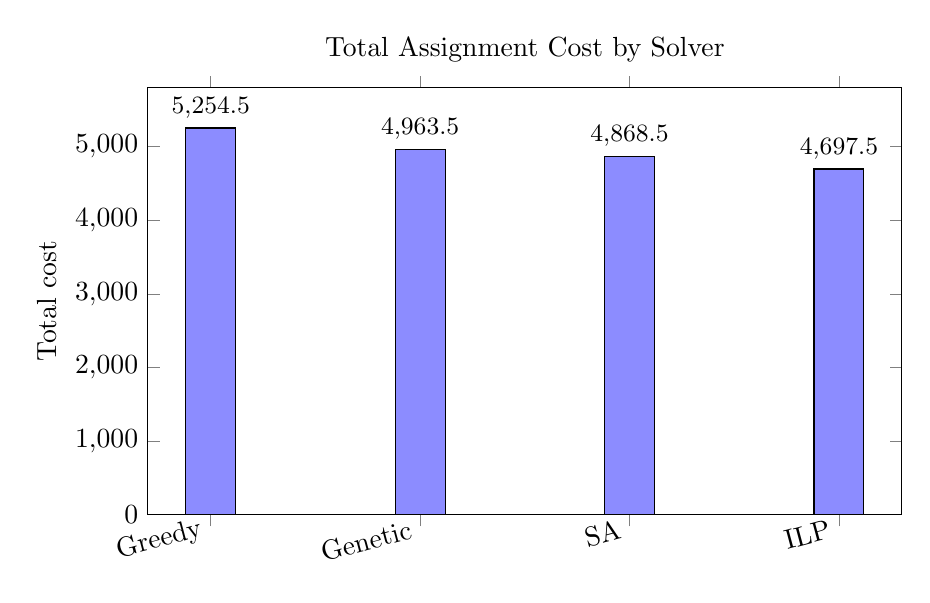
\begin{tikzpicture}
\begin{axis}[
    ybar,
    width=0.92\textwidth,
    height=7cm,
    bar width=18pt,
    ylabel={Total cost},
    symbolic x coords={Greedy,Genetic,SA,ILP},
    xtick=data,
    ymin=0,
    ymax=5800,
    nodes near coords,
    nodes near coords align={vertical},
    every node near coord/.append style={font=\small},
    x tick label style={rotate=15, anchor=east},
    title={Total Assignment Cost by Solver},
]
\addplot[fill=blue!45, draw=black] coordinates {
    (Greedy,5254.5)
    (Genetic,4963.5)
    (SA,4868.5)
    (ILP,4697.5)
};
\end{axis}
\end{tikzpicture}
\caption{Comparison of total assignment cost. Lower values indicate better assignment quality.}
\label{fig:cost}
\end{figure}

\begin{figure}[H]
\centering
\begin{minipage}{0.48\textwidth}
\centering
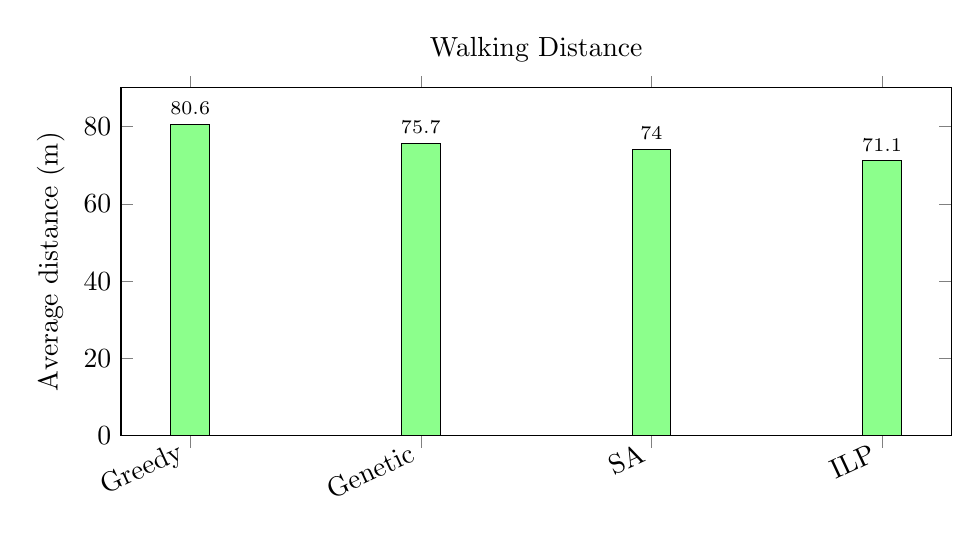
\begin{tikzpicture}
\begin{axis}[
    ybar,
    width=\textwidth,
    height=6cm,
    bar width=14pt,
    ylabel={Average distance (m)},
    symbolic x coords={Greedy,Genetic,SA,ILP},
    xtick=data,
    ymin=0,
    ymax=90,
    nodes near coords,
    every node near coord/.append style={font=\scriptsize},
    x tick label style={rotate=25, anchor=east},
    title={Walking Distance},
]
\addplot[fill=green!45, draw=black] coordinates {
    (Greedy,80.6)
    (Genetic,75.7)
    (SA,74.0)
    (ILP,71.1)
};
\end{axis}
\end{tikzpicture}
\end{minipage}
\hfill
\begin{minipage}{0.48\textwidth}
\centering
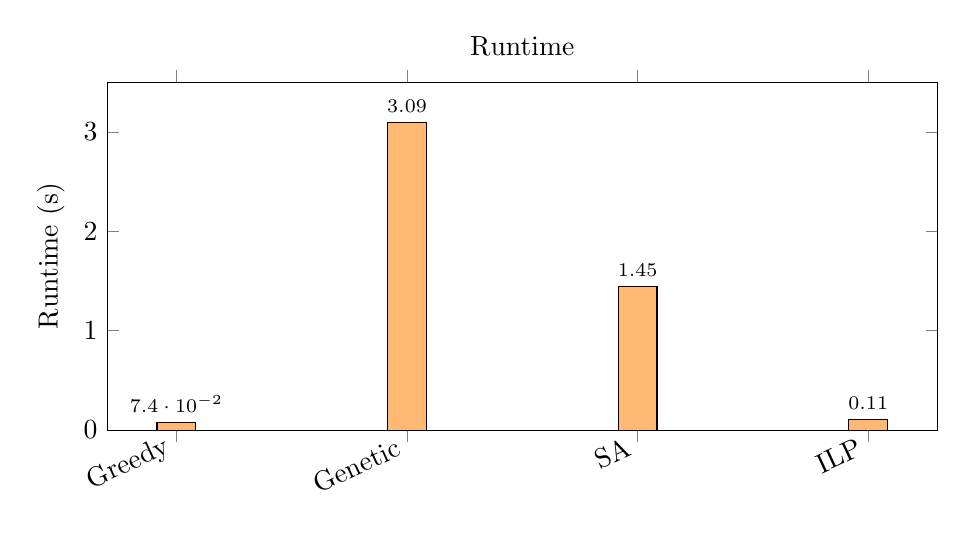
\begin{tikzpicture}
\begin{axis}[
    ybar,
    width=\textwidth,
    height=6cm,
    bar width=14pt,
    ylabel={Runtime (s)},
    symbolic x coords={Greedy,Genetic,SA,ILP},
    xtick=data,
    ymin=0,
    ymax=3.5,
    nodes near coords,
    every node near coord/.append style={font=\scriptsize},
    x tick label style={rotate=25, anchor=east},
    title={Runtime},
]
\addplot[fill=orange!55, draw=black] coordinates {
    (Greedy,0.074)
    (Genetic,3.094)
    (SA,1.447)
    (ILP,0.107)
};
\end{axis}
\end{tikzpicture}
\end{minipage}
\caption{Trade-off between walking distance and runtime. Greedy is fastest, while ILP gives the best distance for this instance.}
\label{fig:distance-runtime}
\end{figure}

\begin{figure}[H]
\centering
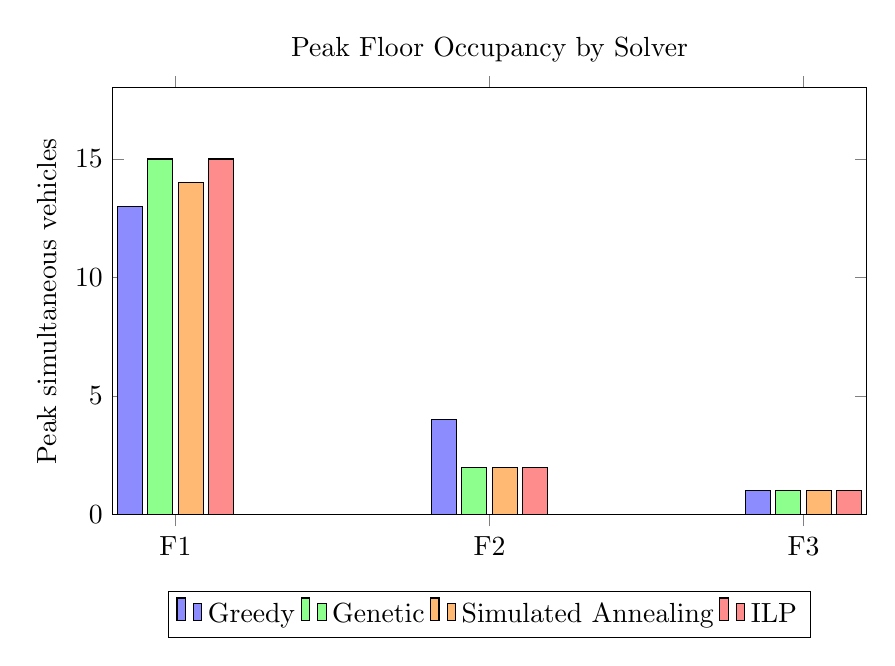
\begin{tikzpicture}
\begin{axis}[
    ybar,
    width=0.92\textwidth,
    height=7cm,
    bar width=9pt,
    ylabel={Peak simultaneous vehicles},
    symbolic x coords={F1,F2,F3},
    xtick=data,
    ymin=0,
    ymax=18,
    legend style={at={(0.5,-0.18)}, anchor=north, legend columns=4},
    title={Peak Floor Occupancy by Solver},
]
\addplot[fill=blue!45, draw=black] coordinates {(F1,13) (F2,4) (F3,1)};
\addplot[fill=green!45, draw=black] coordinates {(F1,15) (F2,2) (F3,1)};
\addplot[fill=orange!55, draw=black] coordinates {(F1,14) (F2,2) (F3,1)};
\addplot[fill=red!45, draw=black] coordinates {(F1,15) (F2,2) (F3,1)};
\legend{Greedy, Genetic, Simulated Annealing, ILP}
\end{axis}
\end{tikzpicture}
\caption{Peak simultaneous occupancy per floor. This metric reflects dynamic occupancy rather than cumulative assignments over the whole simulation.}
\label{fig:occupancy}
\end{figure}

\section{Discussion}

The results show that the ILP method obtains the best solution, with the lowest total cost and lowest average walking distance. This is expected because ILP is an offline exact method and has full knowledge of the vehicle arrival and departure times.

The greedy algorithm is the fastest method, but it produces the highest cost because it makes decisions locally without considering future arrivals.

The genetic algorithm improves the greedy solution, reducing the cost from 5254.5 to 4963.5. Simulated annealing performs even better in this experiment, reaching a cost of 4868.5.

The solution quality ranking is:

\begin{equation}
\text{ILP} < \text{Simulated Annealing} < \text{Genetic Algorithm} < \text{Greedy}
\end{equation}

Since lower cost is better, this means ILP gives the best solution, followed by simulated annealing, then the genetic algorithm, then greedy.

All methods achieved:

\begin{itemize}
    \item 100\% EV satisfaction,
    \item 0\% size violations,
    \item 1.7\% unassigned vehicles.
\end{itemize}

The unassigned rate corresponds to approximately one vehicle out of 60. This can happen because of time overlap, size compatibility, or charger availability constraints.

\section{Validation}

The implementation was validated by running:

\begin{lstlisting}[language=bash]
python main.py
python main.py --no-ga --no-sa --no-ilp
python -m py_compile main.py solver.py instance_gen.py evaluator.py data_loader.py
\end{lstlisting}

The first command runs all solvers. The second command checks that the pipeline can run only the greedy baseline. The third command verifies that all Python files compile successfully.

\section{Limitations}

The main limitations of the current implementation are:

\begin{itemize}
    \item ramp and elevator access capacity are not enforced as hard constraints,
    \item congestion is simplified,
    \item ILP is an offline benchmark and assumes future information is known,
    \item the parking geometry is synthetic,
    \item metaheuristic performance depends on parameter choices.
\end{itemize}

\section{Future Work}

Future improvements may include:

\begin{itemize}
    \item adding hard ramp/elevator capacity constraints,
    \item modeling congestion more realistically,
    \item testing larger benchmark instances,
    \item generating more complex parking layouts,
    \item studying sensitivity to EV charger availability and demand intensity,
    \item producing animated or time-series occupancy visualizations,
    \item comparing additional metaheuristics such as tabu search or ant colony optimization.
\end{itemize}

\section{Conclusion}

This project implemented and compared several optimization approaches for a dynamic multi-level parking assignment problem. The implementation uses real dataset statistics to generate synthetic benchmark instances and evaluates four methods: greedy assignment, genetic algorithm, simulated annealing, and integer linear programming.

The implemented model respects the main constraints of the problem: vehicle assignment, space capacity over time, size compatibility, EV charging requirements, floor capacity, and dynamic arrivals and departures. The results show that heuristic methods improve over the greedy baseline, while ILP provides the best offline benchmark solution.

\end{document}
